\usetikzlibrary{plotmarks}

\begin{figure}[H]
\centering
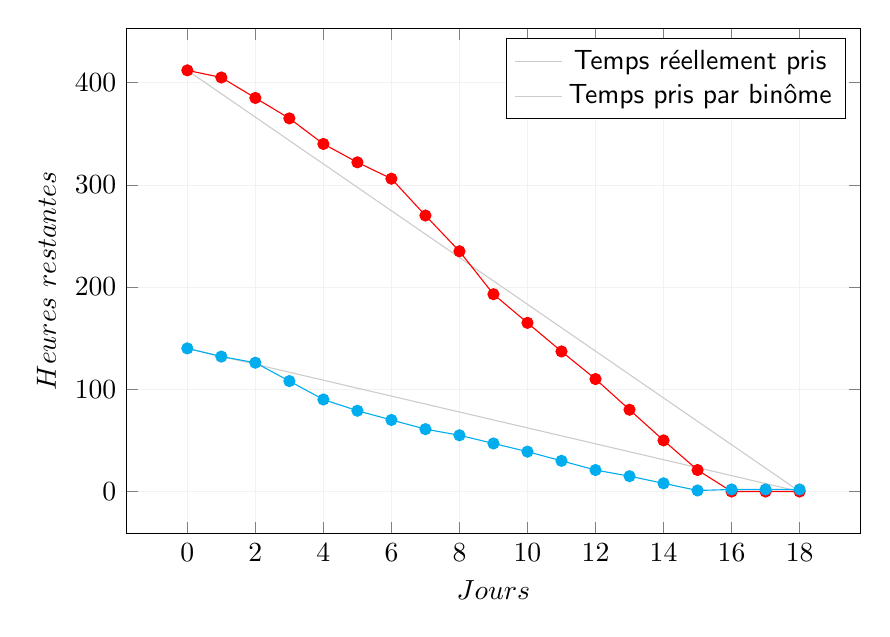
\begin{tikzpicture}[y=.2cm, x=.7cm,font=\sffamily]
\begin{axis}[
xlabel=$Jours$,
ylabel=$Heures\ restantes$,
grid=both,
grid style={line width=.1pt, draw=gray!10},
width=0.9\textwidth,
height=8cm,
%major grid style={line width=.2pt,draw=gray!50},
]
      \addplot[gray!40] plot coordinates {%
(0, 412)
(18, 0)
    };
      \addplot[gray!40] plot coordinates {%
(0, 140)
(18, 0)
    };

    \addplot[mark=*,red] plot coordinates {%
        (0, 412)
        (1, 405)
        (2, 385)
        (3, 365)
        (4, 340)
        (5, 322)
        (6, 306)
        (7, 270)
        (8, 235)
        (9, 193)
        (10, 165)
        (11, 137)
        (12, 110)
        (13, 80)
        (14, 50)
        (15, 21)
        (16, 0)
        (17, 0)
        (18, 0)
    };
    \addlegendentry{Temps réellement pris}

    \addplot[mark=*,cyan] plot coordinates {%
        (0, 140)
        (1, 132)
        (2, 126)
        (3, 108)
        (4, 90)
        (5, 79)
        (6, 70)
        (7, 61)
        (8, 55)
        (9, 47)
        (10, 39)
        (11, 30)
        (12, 21)
        (13, 15)
        (14, 8)
        (15, 1)
        (16, 2)
        (17, 2)
        (18, 2)
    };
    \addlegendentry{Temps pris par binôme}
\end{axis}
\end{tikzpicture}
\caption{Graphique d'avancement - Itération 1}
\label{fig:sprint1-burndown}
\end{figure}
